%! TeX root = openfoam_presentation.tex
\usetheme[framenumber-footline]{Mumbai}



\usepackage[edges]{forest}
\usepackage{listofitems}
\usepackage{mathtools}
\usepackage{siunitx}
\usepackage{tikz}
\usetikzlibrary{3d, calc, perspective}
\usepackage{xparse}



\def\blockmesh{\texttt{blockMesh}}
\def\icofoam{\texttt{icoFoam}}
\def\lapfoam{\texttt{laplacianFoam}}
\def\openfoam{\texttt{OpenFOAM}}
\def\paraview{\texttt{ParaView}}
\def\parafoam{\texttt{paraFoam}}
\newcommand{\defeq}{\coloneqq}
\newcommand{\setitemsep}[1]{\setlength\itemsep{#1}}
\newcommand{\OpenfoamUnitSet}[1]{%
    \readlist*{\units}{#1}
    [\units[1]~\units[2]~\units[3]~\units[4]~\units[5]~\units[6]~\units[7]]
}
\newcommand{\ndnum}[1]{\text{#1}}
\NewDocumentCommand{\pder}{omm}{%
    \IfNoValueTF{#1}{\ensuremath{\frac{\partial #2}{\partial #3}}}{\ensuremath{\frac{\partial^#1 #2}{\partial #3^#1}}}
}
%\newcommand{\pder}[2]{\ensuremath{\frac{\partial #1}{\partial #2}}}




\begin{document}

\title{Introduction to \openfoam}
\author{Vachan Potluri}
\date{April 2023}

{
\setbeamertemplate{footline}{}
\frame{\maketitle}
}

\begin{frame}
    \begin{block}{What}
        \begin{itemize}
            \item CFD software (but without GUI)
            \item \textbf{Open} source \textbf{F}ield \textbf{O}peration \textbf{A}nd \textbf{M}anipulation
            \item Open source $\implies$ source code is given to user
        \end{itemize}
    \end{block}
\onslide<2->
    \begin{figure}
        \includegraphics[width=\linewidth]{opensource_illustration}
    \end{figure}
\onslide<3->
    No GUI $\implies$ hard to learn
    \begin{block}{Why}
        \begin{itemize}
            \item Free
            \item Fast
            \item User customisable: solve any equation you desire
        \end{itemize}
    \end{block}
\onslide<4->
    Let's jump right away into doing some simulations
\end{frame}

\begin{frame}{Case 1}{Heat conduction in a square plate}
    \begin{columns}
        \begin{column}{0.5\linewidth}
            \begin{equation*}
                \pder{T}{t} = D_T \left( \pder[2]{T}{x} + \pder[2]{T}{y} \right)
            \end{equation*}
            \begin{figure}
                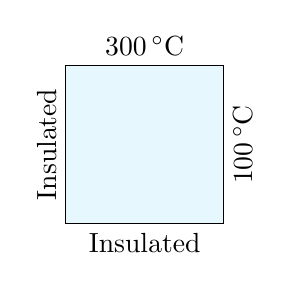
\begin{tikzpicture}[scale=2]
                    \draw [fill=cyan!10] (0,0) -- node [below] {Insulated} (1,0) -- node [rotate=90, below] {\qty{100}{\degreeCelsius}} (1,1) -- node [above] {\qty{300}{\degreeCelsius}} (0,1) -- node [rotate=90, above] {Insulated} cycle;
                \end{tikzpicture}
            \end{figure}
        \end{column}
        \begin{column}{0.5\linewidth}
            Other settings
            \begin{itemize}
                \item $D_T=\qty{1}{m^2/s}$
                \item $L=\qty{2}{m}$
                \item End time \qty{10}{s}
            \end{itemize}
        \end{column}
    \end{columns}
\onslide<2->
    \begin{itemize}
        \item \lapfoam{} is the ``solver'' to be used for heat conduction equation
\onslide<3->
        \item Visualise using \texttt{paraFoam -builtin}
        \begin{itemize}
            \item Mesh representation
            \item Data array selection
            \item Navigating times
            \item Changing color map
        \end{itemize}
    \end{itemize}
\end{frame}

\begin{frame}{\openfoam's simulation setup}
    \begin{columns}
        \begin{column}{0.5\linewidth}
            \begin{block}{Case structure for \lapfoam}
                \begin{figure}
                    \centering
                    \begin{forest}
                        for tree={
                            font=\ttfamily,
                            grow'=0,
                            child anchor=west,
                            parent anchor=south,
                            anchor=west,
                            calign=first,
                            edge path={
                                \noexpand\path [draw, \forestoption{edge}]
                                (!u.south west) +(7.5pt,0) |- node[circle,fill,inner sep=1.25pt] {} (.child anchor)\forestoption{edge label};
                            },
                            before typesetting nodes={
                                if n=1
                                {insert before={[,phantom]}}
                                {}
                            },
                            fit=band,
                            before computing xy={l=15pt},
                        }
                        [case\_name/
                            [0/
                                [T]
                            ]
                            [constant/
                                [physicalProperties]
                                [polyMesh/*]
                            ]
                            [system/
                                [controlDict]
                                [fvSchemes]
                                [fvSolution]
                            ]
                        ]
                    \end{forest}
                \end{figure}
            \end{block}
        \end{column}
        \begin{column}{0.5\linewidth}
            \begin{itemize}
                \setitemsep{1em}
                \item Every simulation is setup using certain ``setting'' files
                \item These files are grouped into 3 folders: \texttt{0/}, \texttt{constant/} and \texttt{system/}
                \item All the setting files are text files
\onslide<2->
                \item Only mandatory files are shown here, there can be additional files also
                \item When a simulation is done, \openfoam{} generates corresponding time files
                \item We will learn about these files by doing some variations of the square plate simulation
            \end{itemize}
        \end{column}
    \end{columns}
\end{frame}

\begin{frame}{Case 1, variation 1}{Change the thermal diffusivity}
    \begin{itemize}
        \setitemsep{1em}
        \item In \texttt{constant/physicalProperties}, you can change $D_T$
\onslide<2->
        \item Things to note
        \begin{itemize}
            \item \texttt{FoamFile} ``header''
            \item Units of $D_T$
            \item Units in \openfoam{} are specified using powers of 7 fundamental units: [\unit{kg} \unit{m} \unit{s} \unit{K} \unit{mol} \unit{A} \unit{cd}]
            \begin{itemize}
                \item \OpenfoamUnitSet{1,1,-2,0,0,0,0} is \unit{kg.m/s^2} $\implies$ force
                \item \OpenfoamUnitSet{0,0,1,0,0,1,0} is \unit{A.s} $\implies$ charge
                \item \OpenfoamUnitSet{1,2,-2,-1,-1,0,0} is \unit{J/mol.K} $\implies$ universal gas constant
            \end{itemize}
        \end{itemize}
\onslide<3->
        \item Try
        \begin{itemize}
            \item Reduce $D_T$ to \qty{0.01}{m^2/s} and see the solution evolution
            \item Can you guess whether the solution will evolve faster or slower?
        \end{itemize}
        \item Tips
        \begin{itemize}
            \item \texttt{foamListTimes -rm} deletes all time folders other than \texttt{0/}
            \item Reload files in \paraview{} by right-clicking
        \end{itemize}
    \end{itemize}
\end{frame}

\begin{frame}{Case 1, variation 2}{Change the boundary conditions}
    \begin{itemize}
        \setitemsep{1em}
        \item In \texttt{0/T} you can set initial condition (IC) and boundary conditions (BCs)
        \item Things to note
        \begin{itemize}
            \item \texttt{internalField} $\implies$ IC
            \item Names of different boundaries
            \item \texttt{type} of different boundaries $\implies$ type of BC
        \end{itemize}
\onslide<2->
        \item Special BC type \texttt{empty}
        \begin{itemize}
            \item By default \openfoam{} does 3d simulations
            \begin{itemize}
                \item Check this in \paraview
            \end{itemize}
            \item \texttt{empty} BC in a direction tells \openfoam{} to not consider that direction
        \end{itemize}
\onslide<3->
        \item Try
        \begin{itemize}
            \item Change bottom BC to \qty{-100}{\degreeCelsius}
            \item Change IC
            \item Do a 1d simulation by setting top and bottom boundaries as \texttt{zeroGradient}
            \begin{itemize}
                \item Verify the solution using ``Plot Over Line'' in \paraview{} or \texttt{gradTx} value
            \end{itemize}
        \end{itemize}
    \end{itemize}
\end{frame}

\begin{frame}{Case 1, variation 3}{Change time settings}
    \begin{itemize}
        \setitemsep{1em}
        \item \texttt{system/controlDict} contains all the main controls of the simulation
        \item Things to note
        \begin{itemize}
            \item \texttt{startFrom}, \texttt{stopAt}
            \item \texttt{startTime}, \texttt{endTime}
            \item \texttt{deltaT}
            \item \texttt{writeControl}, \texttt{writeInterval}
        \end{itemize}
\onslide<2->
        \item For heat conduction equation
        \begin{itemize}
            \item ``Stable'' time step value ($\Delta t_s$) satisfies $D_T \dfrac{\Delta t_s}{\Delta x^2} < 1$
            \item To determine end time ($t_e$) for steady state:
            \begin{equation*}
                t_e \gg \frac{L^2}{D_T} \implies \text{Steady state reached}
            \end{equation*}
        \end{itemize}
\onslide<3->
        \item Try
        \begin{itemize}
            \item Increase $D_T$ to \qty{10}{m^2/s}
            \item For correct simulation, time step also has to be changed
        \end{itemize}
    \end{itemize}
\end{frame}

\begin{frame}{Case 1, variation 4}{Change the mesh}
    \begin{itemize}
        \setitemsep{1em}
        \item Multiple ways to create mesh in \openfoam
        \begin{itemize}
            \item Create in a different software (e.g. ANSYS) and import to \openfoam
            \item Use \openfoam's tools to create mesh
        \end{itemize}
        \item<2-> \blockmesh{} is one such tool in \openfoam{} to create meshes
        \item<3-> \blockmesh{} reads an additional file \texttt{system/blockMeshDict} to create mesh
        \item<4-> \texttt{system/blockMeshDict} has 3 components
        \begin{enumerate}
            \item Specify points or vertices
            \item Create ``blocks'' using these vertices
            \item Define boundaries using the vertices
        \end{enumerate}
    \end{itemize}
\end{frame}

\begin{frame}
    \begin{itemize}
        \setitemsep{1em}
        \item \openfoam{} defines a local coordinate system (LCS) for every block
        \item Blocks are created using a list of points $(p_0~p_1~p_2~p_3~p_4~p_5~p_6~p_7)$ ordered in a specific way
        \begin{enumerate}
            \item Point $p_0$ is the origin of LCS
            \item Line $p_0$-$p_1$ is along $x_1$ direction
            \item Line $p_1$-$p_2$ is along $x_2$ direction
            \item Points $p_0$-$p_3$ define plane $x_3=0$
            \item Points $p_4$-$p_7$ are obtained by translating points $p_0$-$p_3$ in $x_3$ direction
        \end{enumerate}
    \end{itemize}
    \begin{figure}
        \centering
        Suppose a block is defined using $(p_0~p_1~p_2~p_3~p_4~p_5~p_6~p_7)$.\\
        Which one of these is correct?\\[0.5em]
        \includegraphics[width=0.8\linewidth]{blockmesh_ordering}
    \end{figure}
\end{frame}

\begin{frame}
    \begin{itemize}
        \setitemsep{1em}
        \item Boundaries are defined using a list of points such that right hand thumb rule points outward the block
        \item The boundary names in \texttt{system/blockMeshDict} and \texttt{0/T} must match
\onslide<2->
        \item Try
        \begin{itemize}
            \item Increasing mesh resolution
            \item Using mesh grading
            \item Changing geometry
        \end{itemize}
        \item Tips
        \begin{itemize}
            \item Run \texttt{blockMesh} command to update mesh
            \item Run \texttt{checkMesh} command to check if the mesh has no issues
            \item You can view different mesh regions (e.g. boundaries) individually in \paraview
        \end{itemize}
    \end{itemize}
\end{frame}

\begin{frame}{Case 2}{Heat conduction in an L-clamp}
    \begin{columns}
        \begin{column}{0.5\linewidth}
            \begin{figure}
                \centering
                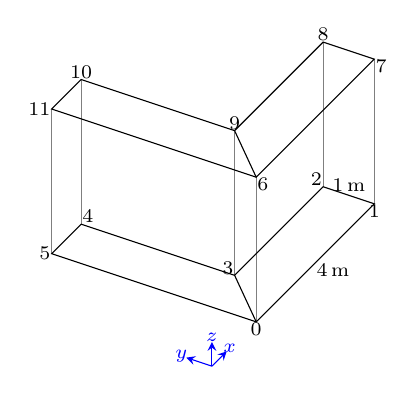
\begin{tikzpicture}[3d view={-60}{35.26}, >=stealth, inner sep=0.25pt, font=\scriptsize, scale=0.75]
                    \begin{scope}[shift={(-1.5,0,0)}, blue, scale=0.5]
                        \draw [->] (0,0,0) -- (1,0,0) node [pos=1.2] {$x$};
                        \draw [->] (0,0,0) -- (0,1,0) node [pos=1.2] {$y$};
                        \draw [->] (0,0,0) -- (0,0,1) node [pos=1.2] {$z$};
                    \end{scope}
                    
                    \begin{scope}[canvas is xy plane at z=0]
                        \draw (0,0) node [below] {0} -- node [anchor=north west] {\qty{4}{m}} (4,0) node [below] {1} -- node [above=1pt] {\qty{1}{m}} (4,1) node [anchor=south east] {2} -- (1,1) node [anchor=south east] {3} -- cycle;
                        \draw (1,1) -- (1,4) node [anchor=south west] {4} -- (0,4) node [left] {5} -- (0,0);
                    \end{scope}
                    
                    \begin{scope}[canvas is xy plane at z=3]
                        \draw (0,0) node [anchor=north west] {6} -- (4,0) node [anchor=north west] {7} -- (4,1) node [above] {8} -- (1,1) node [above] {9} -- cycle;
                        \draw (1,1) -- (1,4) node [above] {10} -- (0,4) node [left] {11} -- (0,0);
                    \end{scope}
                    
                    \foreach \p in {(0,0,0), (4,0,0), (4,1,0), (1,1,0), (0,4,0), (1,4,0)} {%
                        \draw [opacity=0.5] \p -- +(0,0,3);
                    }
                \end{tikzpicture}
            \end{figure}
            \begin{itemize}
\onslide<2->
                \item This geometry can be constructed using two blocks
                \begin{enumerate}
                    \item Block 1: $(p_0 ~ p_1 ~ p_2 ~ p_3 ~ p_6 ~ p_7 ~ p_8 ~ p_9)$
                    \item Block 2: $(p_0 ~ p_3 ~ p_4 ~ p_5 ~ p_6 ~ p_9 ~ p_{10} ~ p_{11})$
                \end{enumerate}
            \end{itemize}
        \end{column}
        \begin{column}{0.5\linewidth}
            \begin{itemize}
\onslide<3->
                \item BCs
                \begin{itemize}
                    \item One end $(p_4 ~ p_5 ~ p_{11} ~ p_{10})$ of clamp at \qty{100}{\degreeCelsius}
                    \item Other end $(p_1 ~ p_2 ~ p_8 ~ p_7)$ at \qty{0}{\degreeCelsius}
                    \item All other boundaries insulated
                    \item \texttt{empty} BC for top and bottom planes
                \end{itemize}
	            \item Tip: you can see the mesh in \paraview{} without running the simulation
\onslide<4->
                \item Use $D_T=\qty{1}{m^2/s}$; set end time and time step accordingly
                \begin{gather*}
                    D_T \frac{\Delta t_s}{\Delta x^2} \le 1\\
                    t_e \gg \frac{L^2}{D_T}
                \end{gather*}
            \end{itemize}
        \end{column}
    \end{columns}
\end{frame}

\begin{frame}{Case 3}{Lid driven cavity}
    \vspace{-1em}
    \begin{columns}[T]
        \begin{column}{0.3\linewidth}
            \begin{figure}
                \centering
                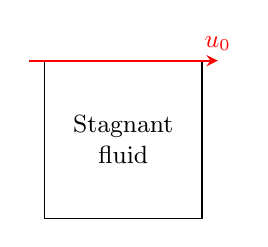
\begin{tikzpicture}[scale=2, >=stealth, font=\small]
                    \draw (0,0) -- ++(0,-1) -- ++(1,0) -- ++(0,1);
                    \draw [thick, red, ->] (-0.1,0) -- +(1.2,0) node [above] {$u_0$};
                    \node [align=center] at (0.5,-0.5) {Stagnant\\fluid};
                \end{tikzpicture}
\onslide<3->
                \begin{forest}
                    for tree={
                        font=\ttfamily\scriptsize,
                        grow'=0,
                        child anchor=west,
                        parent anchor=south,
                        anchor=west,
                        calign=first,
                        edge path={
                            \noexpand\path [draw, \forestoption{edge}]
                            (!u.south west) +(7.5pt,0) |- node[circle,fill,inner sep=0.75pt] {} (.child anchor)\forestoption{edge label};
                        },
                        before typesetting nodes={
                            if n=1
                            {insert before={[,phantom]}}
                            {}
                        },
                        fit=band,
                        before computing xy={l=15pt},
                        s sep=2pt,
                    },
                    [case\_name/
                        [0/
                            [p, red]
                            [U, red]
                        ]
                        [constant/
                            [physicalProperties]
                            [polyMesh/*]
                        ]
                        [system/
                            [controlDict]
                            [fvSchemes]
                            [fvSolution]
                        ]
                    ]
                \end{forest}
            \end{figure}
        \end{column}
        \begin{column}{0.7\linewidth}
\onslide<1->
            \begin{gather*}
                \pder{u}{x} + \pder{v}{y} = 0\\
                \pder{u}{t} + u \pder{u}{x} + v \pder{u}{y} = -\pder{(p/\rho)}{x} + \nu \left( \pder[2]{u}{x} + \pder[2]{u}{y} \right)\\
                \pder{v}{t} + u \pder{v}{x} + v \pder{v}{y} = -\pder{(p/\rho)}{y} + \nu \left( \pder[2]{v}{x} + \pder[2]{v}{y} \right)
            \end{gather*}
            \begin{itemize}
                \setitemsep{0.5em}
\onslide<2-> 
                \item \icofoam{} is one solver for ``transient laminar'' incompressible flow
                \begin{itemize}
\onslide<4->
                    \item \texttt{p} in \icofoam{} is $p/\rho$
                \end{itemize}
\onslide<5->
                \item We will setup this case from scratch using \openfoam's ``tutorial cases''
                \item And learn some techniques in \paraview
                \begin{itemize}
                    \item Extracting 2d slice of a 3d domain
                    \item Plot over line
                    \item Visualising streamlines
                \end{itemize}
            \end{itemize}
        \end{column}
    \end{columns}
\end{frame}

\begin{frame}{Case 4}{Incompressible flat plate boundary layer}
    \begin{columns}
        \begin{column}{0.5\linewidth}
            Incompressible flow simulation of air over a flat plate
            \begin{gather*}
                \rho_\infty = \qty{0.09719}{kg/m^3}, ~ u_\infty = \qty{149.3}{m/s}\\
                p_o = \qty{63.71}{kPa}, ~ \nu = \qty{1.493e-4}{m^2/s}
            \end{gather*}
            \begin{figure}
                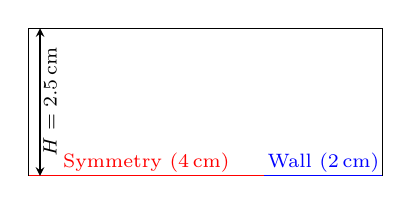
\begin{tikzpicture}[font=\scriptsize, scale=0.75, >=stealth, inner sep=1pt]
                    \draw [red] (-4,0) -- node [above] {Symmetry (\qty{4}{cm})} (0,0);
                    \draw [blue] (0,0) -- node [above] {Wall (\qty{2}{cm})} (2,0);
                    \draw (2,0) -- (2,2.5) -- (0,2.5) -- (-4,2.5) -- (-4,0);
                    \draw [<->] (-3.8,0) -- node [rotate=90, below] {$H=\qty{2.5}{cm}$} +(0,2.5);
                \end{tikzpicture}
                \\[1em]
\onslide<3->
                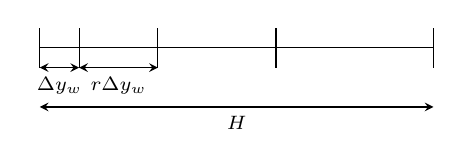
\begin{tikzpicture}[scale=5, >=stealth, font=\scriptsize]
                    \draw (0,0) -- (1,0);
                    \foreach \x in {0,0.1,0.3,0.6,1} {%
                        \draw (\x,-0.05) -- +(0,0.1);
                    }
                    \draw [<->] (0,-0.05) -- node [below] {$\Delta y_w$} +(0.1,0);
                    \draw [<->] (0.1,-0.05) -- node [below] {$r \Delta y_w$} (0.3,-0.05);
                    \draw [<->] (0,-0.15) -- node [below] {$H$} +(1,0);
                \end{tikzpicture}
            \end{figure}
        \end{column}
        \begin{column}{0.5\linewidth}
            \begin{itemize}
\onslide<2->
                \item Estimate BL thickness
                \begin{equation*}
                    \frac{\delta}{x} = \frac{5}{\sqrt{\ndnum{Re}_x}} \approx \qty{0.7}{mm}
                \end{equation*}
\onslide<3->
                \item Use $\Delta y_w \approx \qty{0.1}{mm}$ and grade the mesh away from wall
                \begin{equation*}
                    \frac{H}{\Delta y_w} = \frac{r^n-1}{r-1}
                \end{equation*}
\onslide<4->
                \item Also grade in $x$ direction to have nearly square cells at leading edge
\onslide<5->
                \item Time step and end time:
                \begin{equation*}
                    \frac{u \Delta t_s}{\Delta x} < 1,~
                    t_e \gg \frac{L}{u_\infty}
                \end{equation*}
            \end{itemize}
        \end{column}
    \end{columns}
\end{frame}

\begin{frame}
    \begin{itemize}
        \setitemsep{0.5em}
        \item \openfoam{} has many ``post-processing'' tools
        \item Post-processing is what you do after a simulation
\onslide<2->
        \item Suppose we wish to compare these results with Blasius solution
        \begin{gather*}
            c_f \defeq \frac{\tau_w}{\frac{1}{2} \rho_\infty u_\infty^2} = \frac{0.664}{\sqrt{\ndnum{Re}_x}}\\
            \delta_2 \defeq \int_{0}^{\infty} \frac{u}{u_\infty} \left( 1-\frac{u}{u_\infty} \right) = 0.665 \sqrt{\frac{\nu x}{u_\infty}}
        \end{gather*}
\onslide<3->
        \item We need two things
        \begin{enumerate}
            \item Compute shear stress from velocity data
            \item Obtain the simulation data on wall and at a given $x$ location
        \end{enumerate}
\onslide<4->
        \item Use \texttt{postProcess -func "grad(U)"} for the first
\onslide<5->
        \item For the second, use \texttt{postProcess -func -<filename>} with the corresponding file \texttt{system/}
        \begin{itemize}
            \item Alternatively, \paraview{} can be used to export ``Plot Over Line'' data
        \end{itemize}
    \end{itemize}
\end{frame}

\end{document}